\chapter{Physical Model}
\section{Manufacturing}
\subsection{3D Printing}

All of the custom modeled parts were 3D printed with PLA on a Creality Ender 3 Pro. This allowed them to be manufactured quickly and accurately. However, 3D printing is not perfect. When the plastic exits the nozzle of the printer, it expands, causing part tolerances to be off by a few hundredths of an inch. This is a difference maker in whether or not two parts will fit properly. This is especially troublesome when the prints take 12+ hours to print and need to be reprinted. A technique used to work around this issue was to slice out a piece of the part where the dimensions mattered and print that first. If it doesn't fit, the part can be reprinted at a fraction of the time and material cost. This allows for much faster tolerance iteration. Once the tolerances have been tuned, the full part is printed and fits just as planned.
\begin{figure}[h]
    \centering
    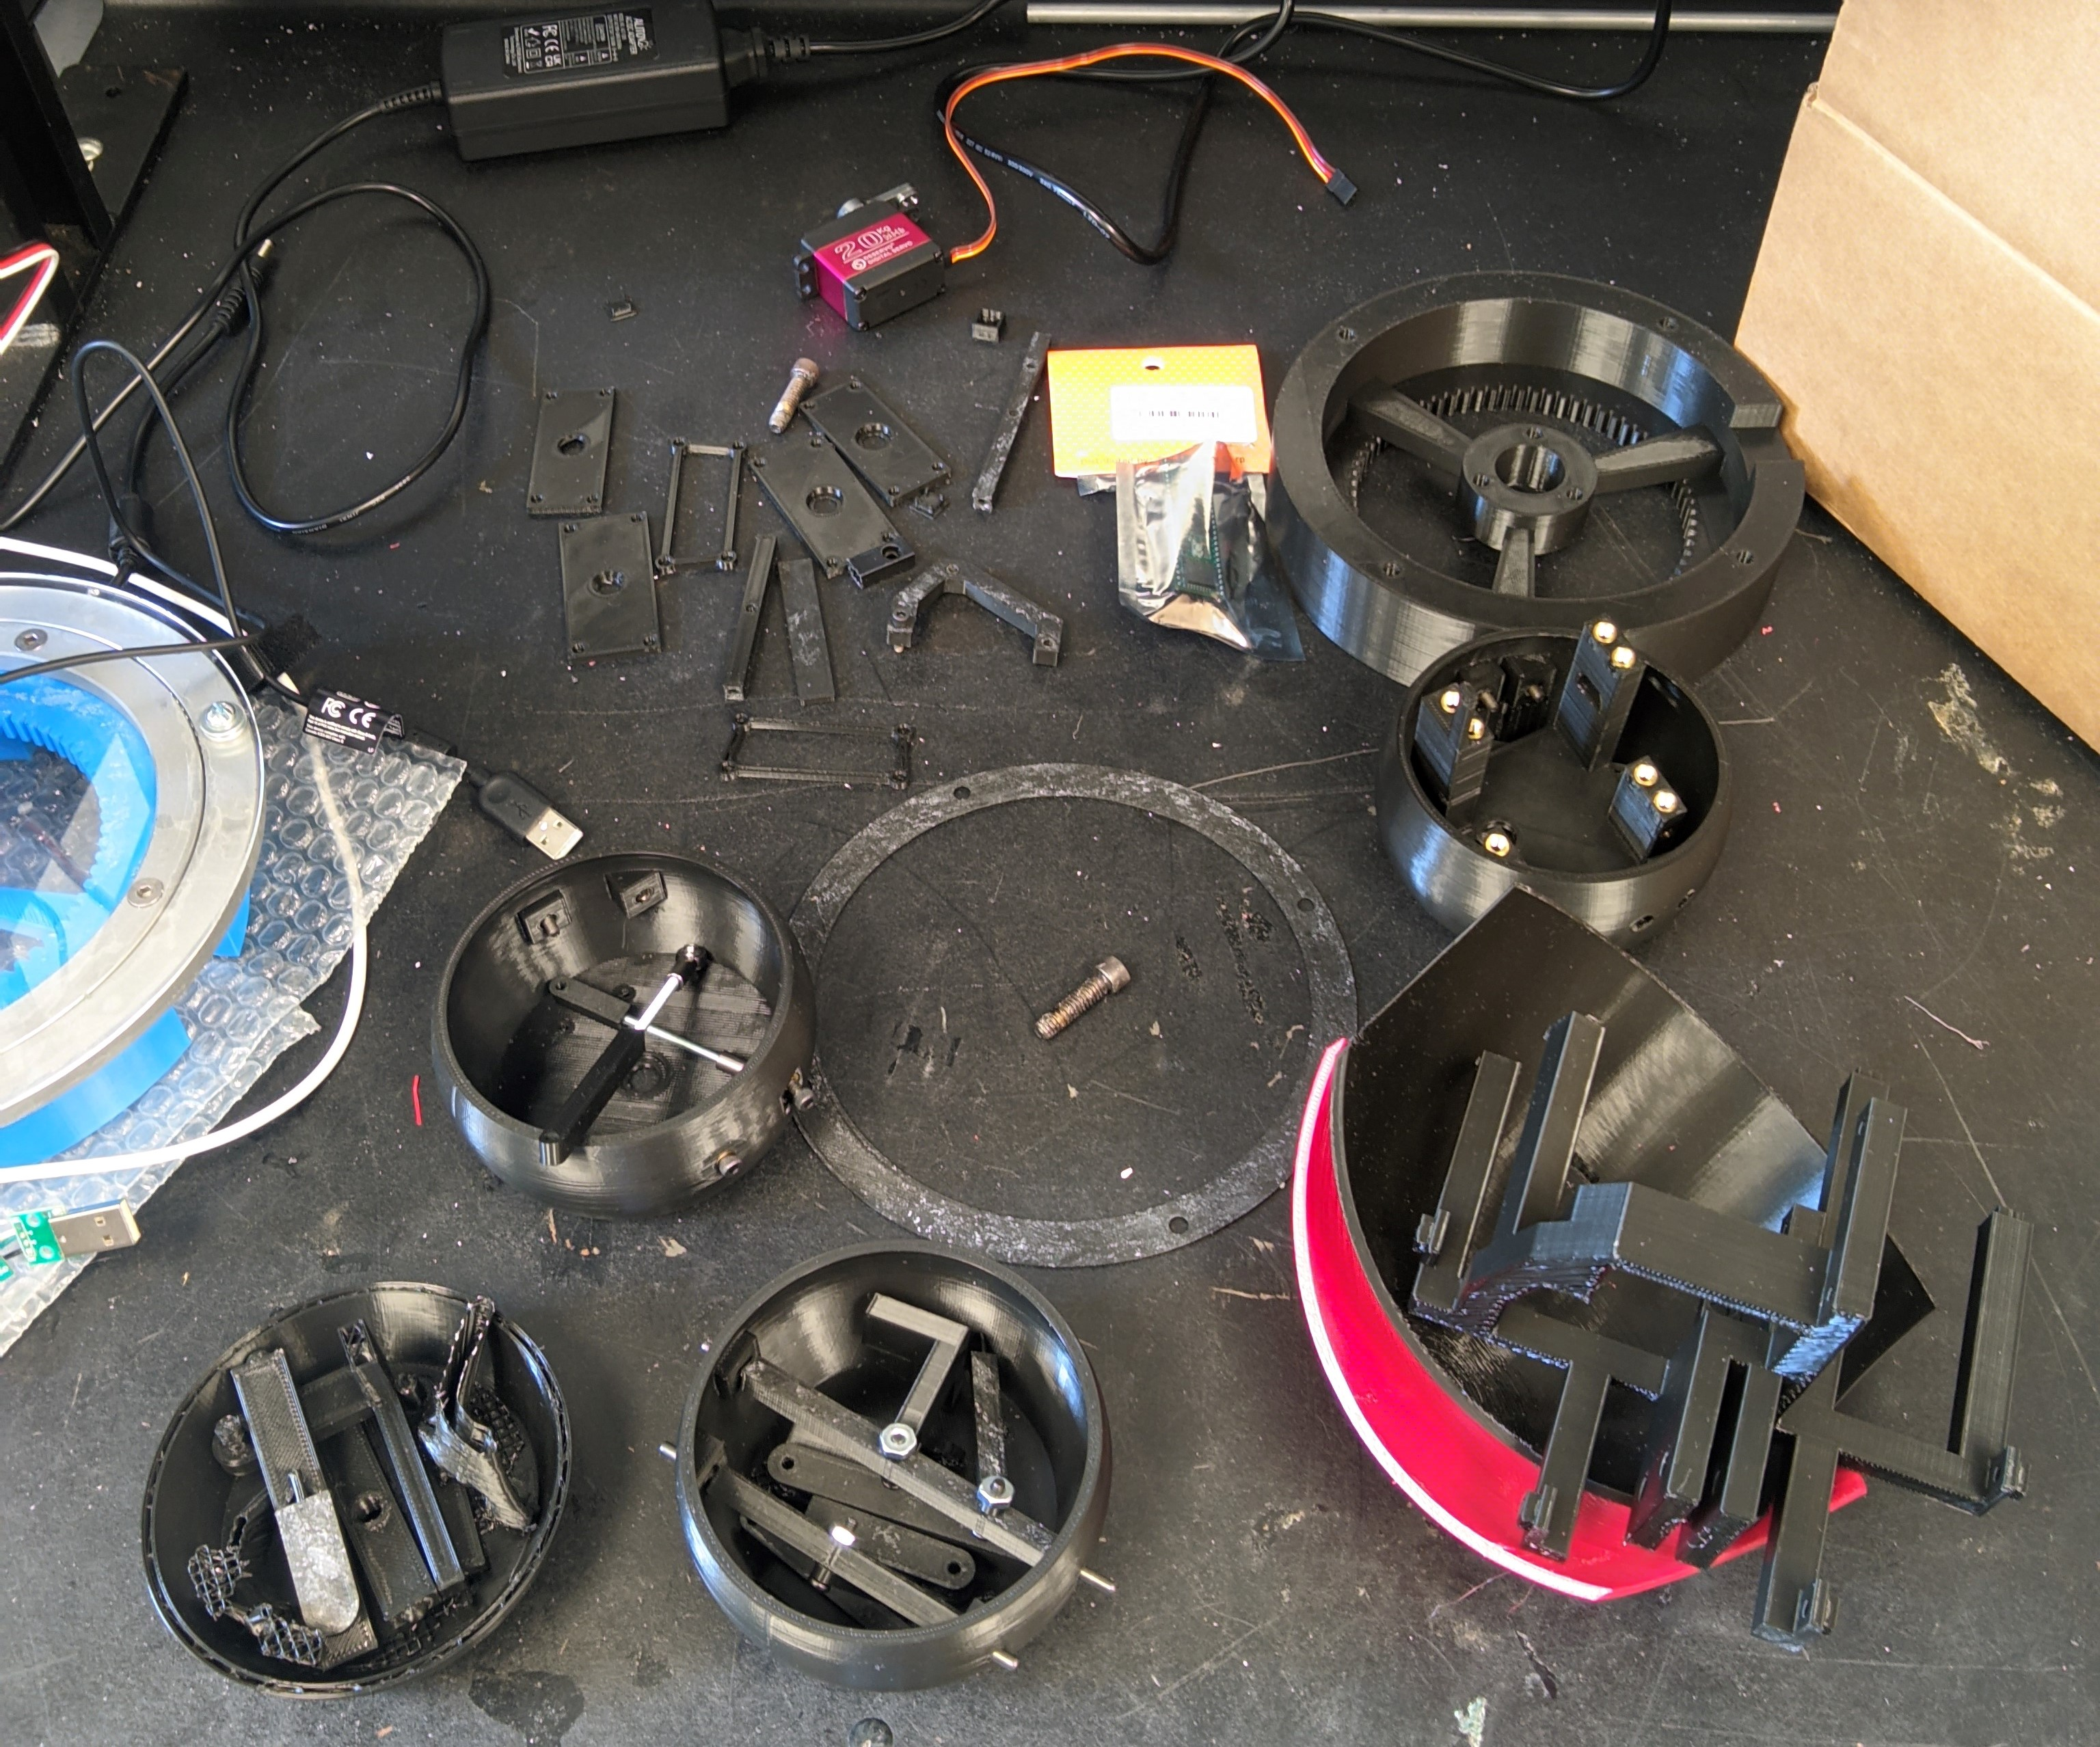
\includegraphics[width=0.5\linewidth]{Thesis/ch3/scrap.jpg}
    \caption{Various failed parts that had to be redesigned.}
    \label{fig:trash-parts}
\end{figure}
\subsection{Aluminum Body}
The part for the body was designed entirely 2-dimensional for CNC milling purposes. The body was CNC milled out of an 1/8'' thick aluminum sheet. A screenshot of the CNC setup in Creo is shown in Figure \ref{fig:mfg}. The part was made out of aluminum because of its slender shape while also bearing the load of the entire head assembly on top of it. A 3D printed part may have not been rigid enough or too weak to hold the weight, although it would have been easier to manufacture. 3D printing is great for a lot of things, but this was a job for the CNC mill.
\begin{figure}[h]
    \centering
    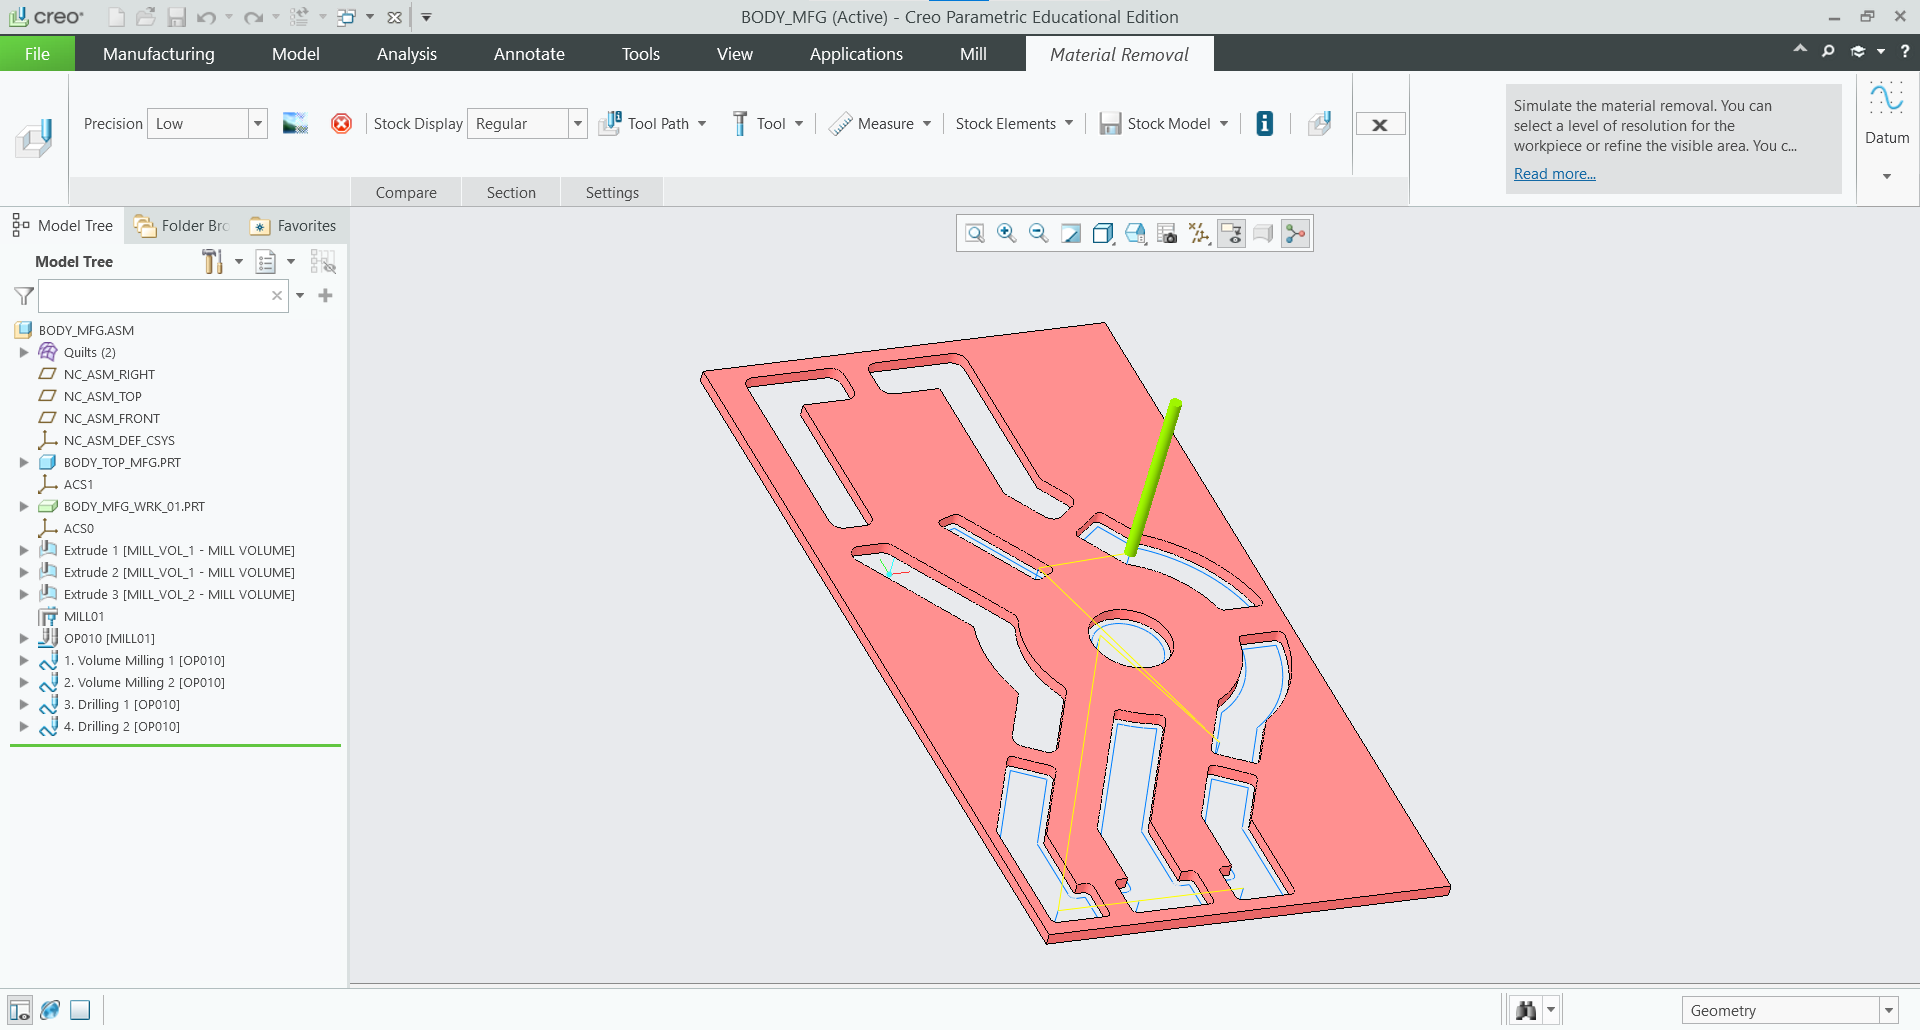
\includegraphics[width=0.6\linewidth]{Thesis/ch3/mfg.png}
    \caption{Screenshot of making the file in Creo to be sent to the CNC machine for manufacturing the body.}
    \label{fig:mfg}
\end{figure}
The aluminum body was secured to the base with 4 $90^\circ$ brackets. These were cut out of a 0.75''x0.75'' piece of L channel stock and drilled on the milling machine to position the holes properly. Figure \ref{fig:bracket_drw} shows the drawing used as a reference to mill and cut the four brackets.

\begin{figure}[h]
    \centering
    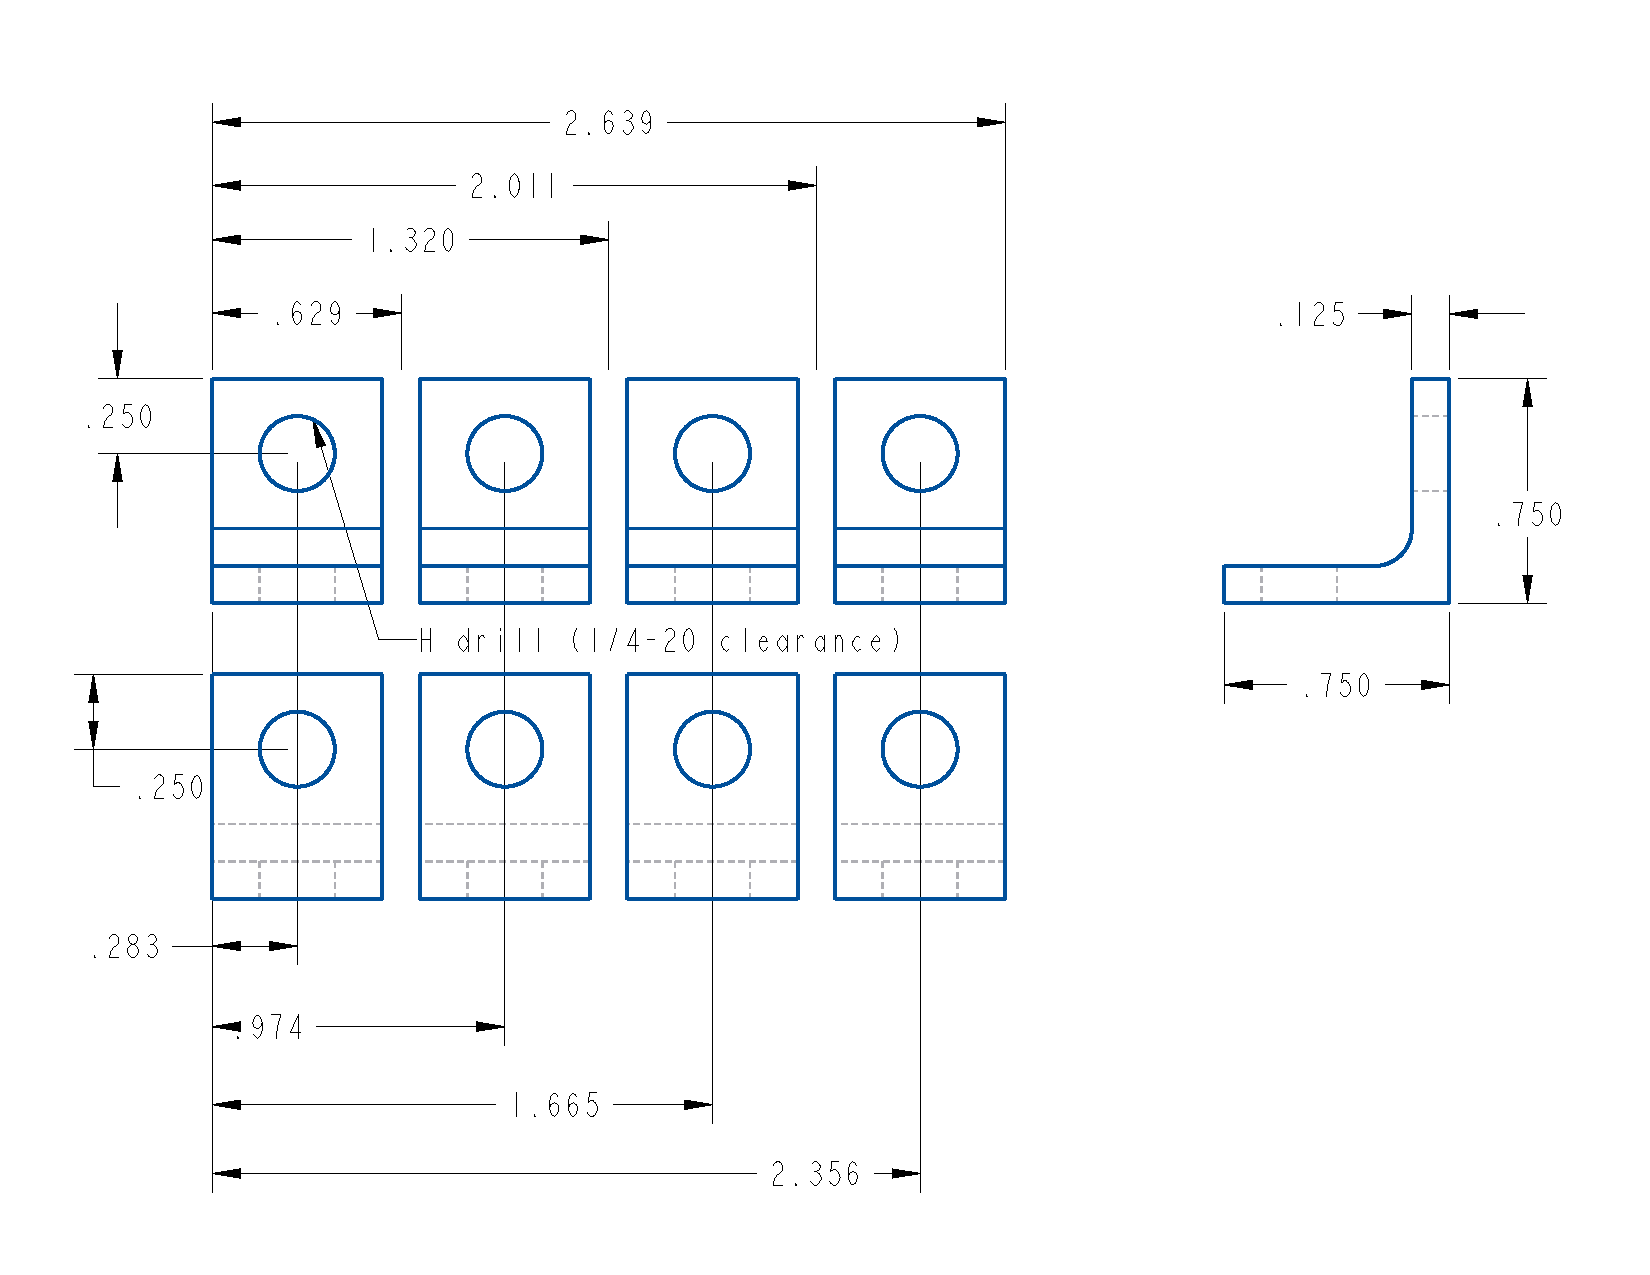
\includegraphics[width=0.6\linewidth]{Thesis/ch3/bracket_drw2.pdf}
    \caption{Drawing used for manufacturing the four metal brackets connecting the body to the base.}
    \label{fig:bracket_drw}
\end{figure}

\subsection{Acrylic Base}
The base was laser cut out of a sheet of 1/8'' thick clear acrylic. This material was chosen for aesthetic reasons and for its ability to be laser cut, which speeds up manufacturing time significantly.

A lazy susan bearing was used for the base to allow it to rotate freely. This is a common bearing used in turntables, where there are steel balls outlining the perimeter of the circle which reduces the friction while rotating the two concentric circles. The lazy susan bearing was an essential part in making the robot spin around its base without requiring a large and powerful stepper motor.

\section{Finishing Parts}
Another aesthetic choice for the product was painting the four plates used in the head assembly as well as the eyeball part. 3D printing produces layer lines in a part, which is fine for prototyping, but for a final model these are undesirable, especially in round parts where layers are more apparent. The parts were first treated with a layer of Bondo filler putty, which filled in some layer lines and parts of the print that had poor surface finishes. The filler putty was then sanded with incrementing grits of sandpaper to smooth out the surface of the dried putty. This process was repeated several times until most of the peaks and valleys were smoothed out. After this, a thick layer of automotive filler primer was applied to the parts to further smooth out the parts and prepare the surfaces for painting. The filler primer has a passive smoothing effect because of the surface tension of the liquid, plus it is very easy to sand. The surfaces were brought up to 400 grit before getting ready to paint. The shells were painted white, while the eyeball was painted black. These colors were chosen to mimic the colors of an eyeball. Figure \ref{fig:manufact} shows three intermediary pictures taken throughout this process.
\begin{figure}
\centering
\begin{subfigure}{0.3\textwidth}
    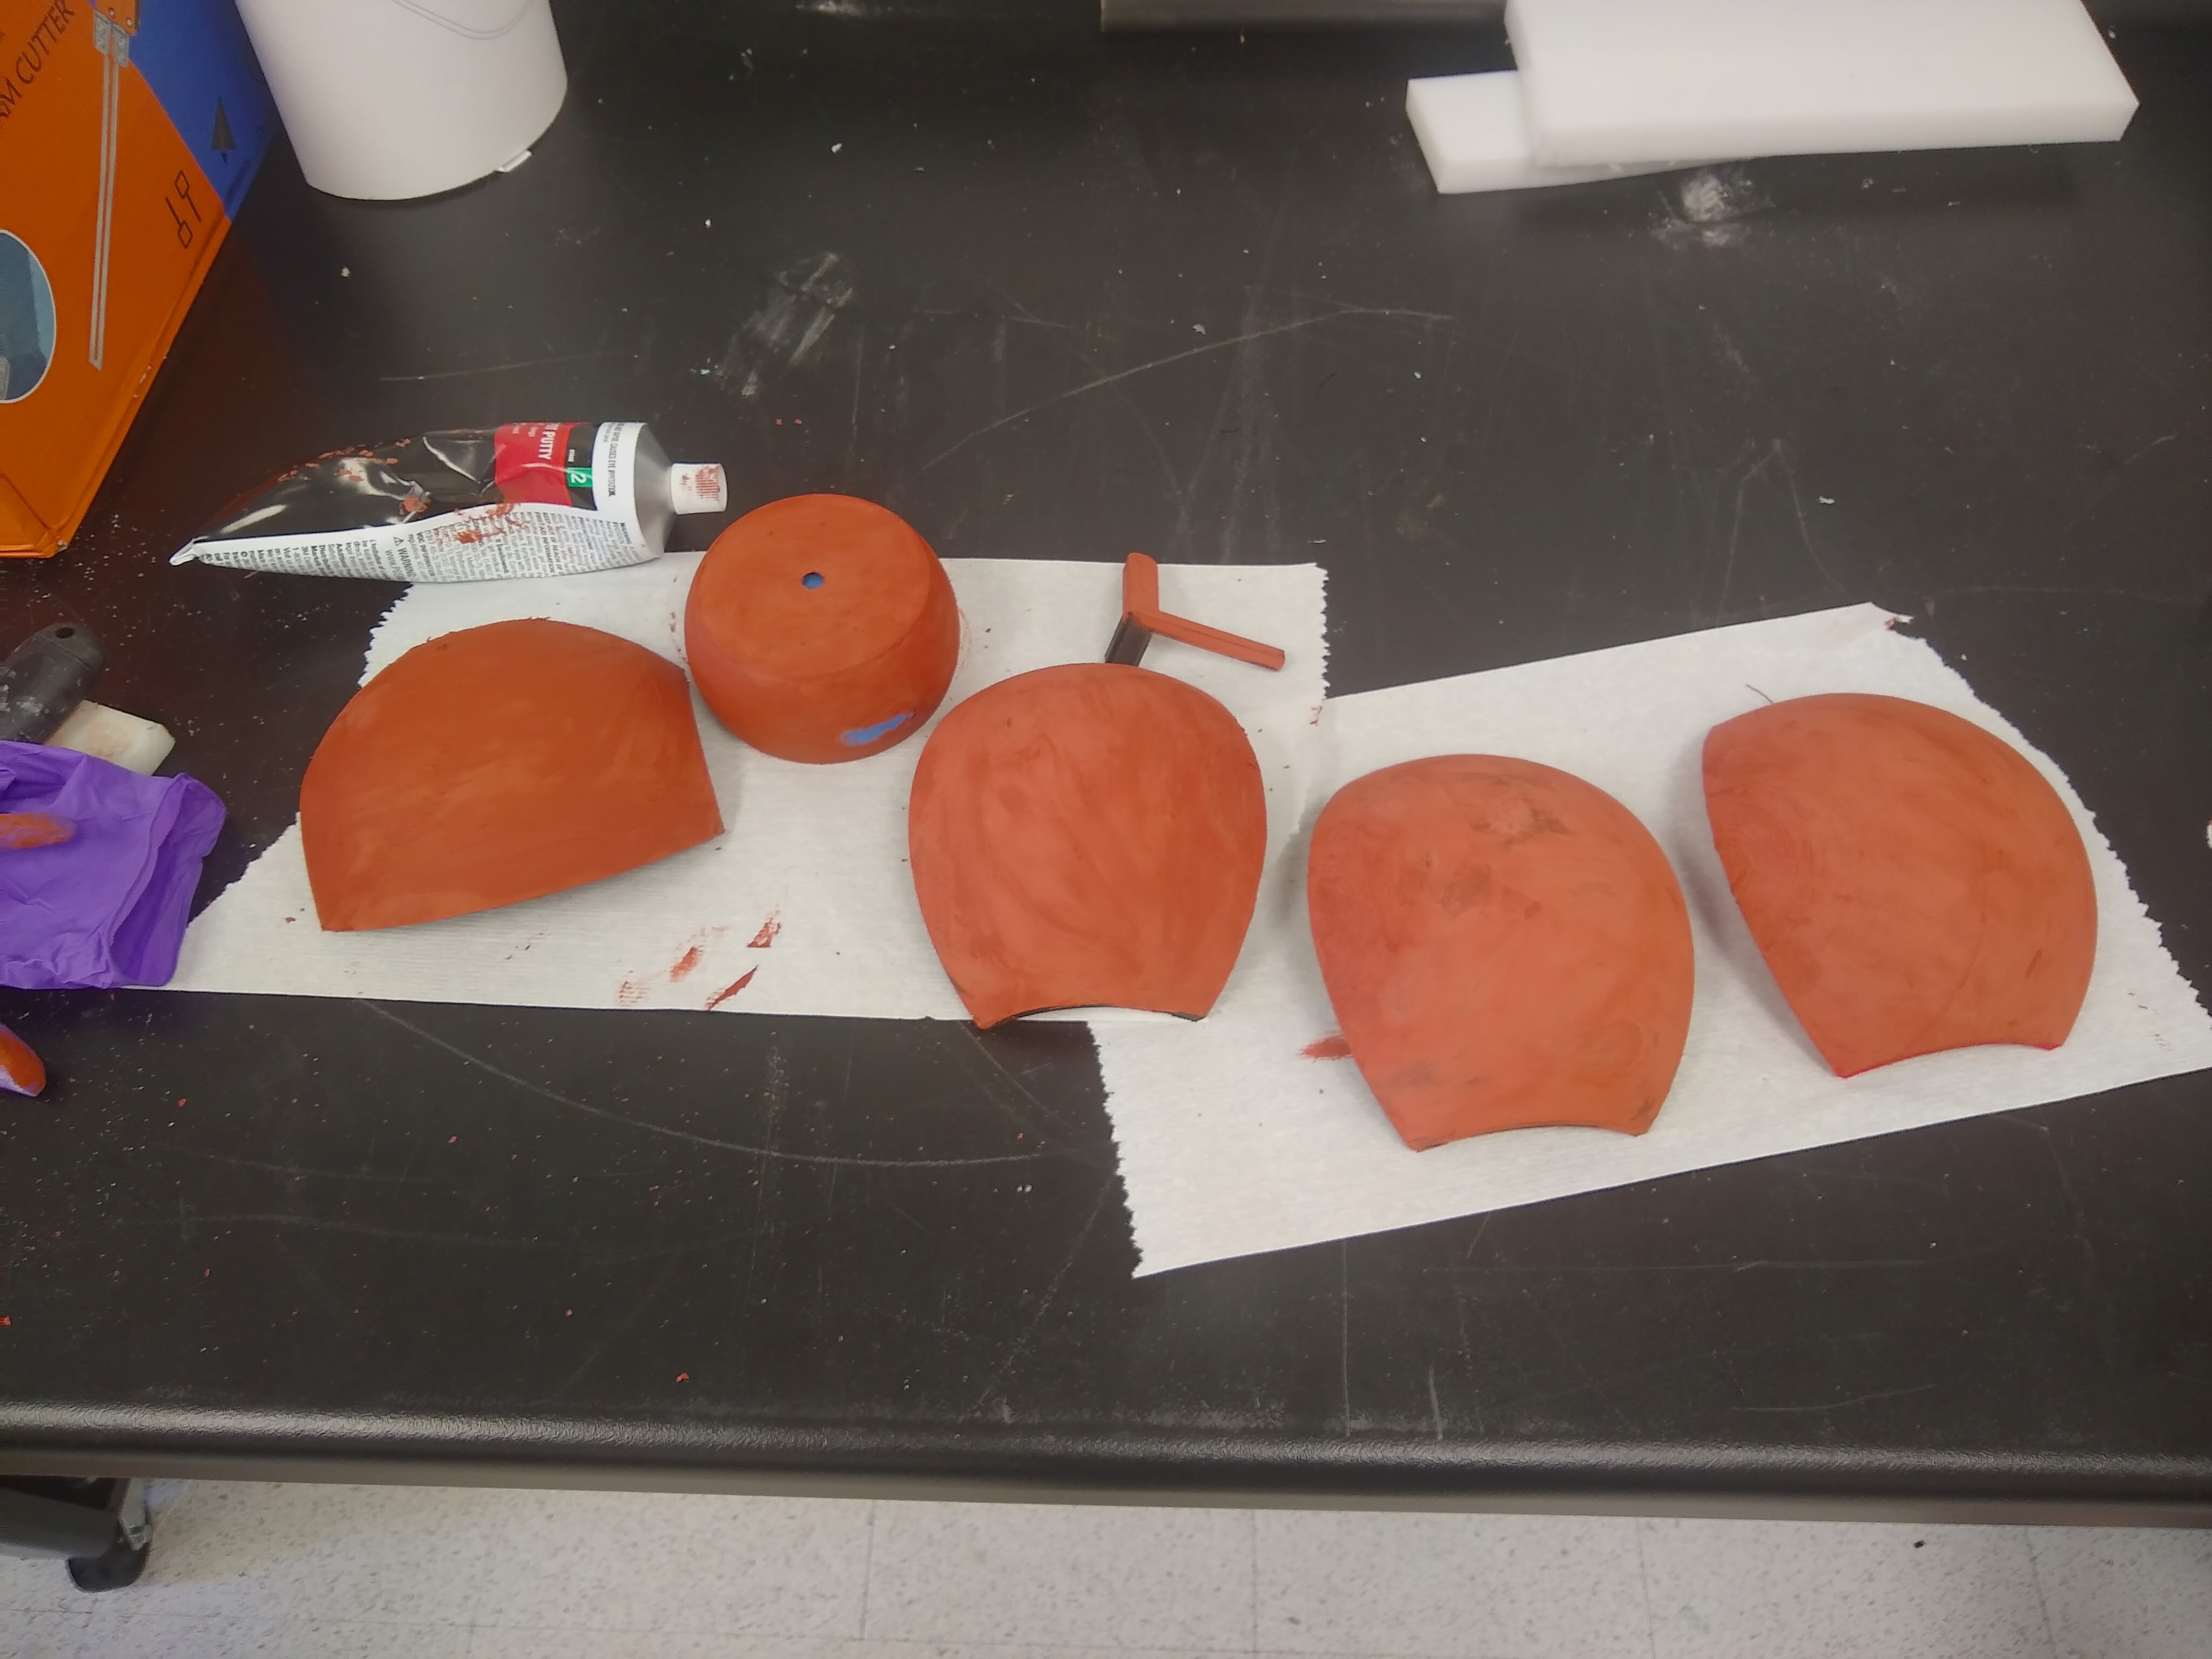
\includegraphics[width=\textwidth]{Thesis/ch3/manufact-1.jpg}
    \caption{Filler putty application}
\end{subfigure}
\hfill
\begin{subfigure}{0.3\textwidth}
    \rotatebox{180}{\includegraphics[width=\textwidth]{Thesis/ch3/manufact-2.jpg}}
    \caption{Filler Primer + sanding}
\end{subfigure}
\hfill
\begin{subfigure}{0.3\textwidth}
    \rotatebox{180}{\includegraphics[width=\textwidth]{Thesis/ch3/manufact-3.jpg}}
    \caption{Spray Painting}
\end{subfigure}
\caption{Process of finishing parts}
\label{fig:manufact}
\end{figure}

\section{Mounting Components}
The head assembly was designed to accommodate the microcontroller, servos, and most of the wiring. This was done to keep a clean look to the robot. An image of the inside of the head can be seen in Figure \ref{fig:servo-shot}. The servos are mounted onto the mounting block with 8-32 screws. They are held in by heat set threaded inserts, which allows for metal threads to be added to a 3D printed part. This provides a strong metal screw hole, as opposed to tapping the plastic itself. To mount the camera, existing geometry of the product was leveraged. The camera enclosure is essentially a plastic box held together by four screws on the front face. By removing this front face, we can reuse these screw holes as mounting geometry, replacing the face of the camera enclosure with the front face of the eyeball. The eyeball part was designed such that the existing screws could mount the camera. The tolerances on such a small part were a challenge, so the previously mentioned iteration technique was used to get the part to fit properly. The Teensy daughter board was mounted with 5-40 screws, shown in Figure \ref{fig:teensy-shot}. These components are all mounted with screws, which was an an important consideration throughout the design process. This was to allow for the robot to be completely disassembled for troubleshooting and replacing broken parts.

\begin{figure}
    \centering
    \begin{subfigure}{0.4\linewidth}
        \rotatebox{270}{\includegraphics[width=\linewidth]{Thesis/appendix/photos/innerds-1.jpg}}
        \caption{}
        \label{fig:servo-shot}
    \end{subfigure}
    \begin{subfigure}{0.4\linewidth}
        \rotatebox{270}{\includegraphics[width=\linewidth]{Thesis/appendix/photos/innerds-left.jpg}}
        \caption{}
        \label{fig:teensy-shot}
    \end{subfigure}
    \caption{View of the mounted components inside the head.}
    \label{fig:mounted}
\end{figure}

\section{Final Model}
The final model completed and assembled is shown in Figure \ref{fig:final_model}.
\begin{figure}[h!]
    \centering
    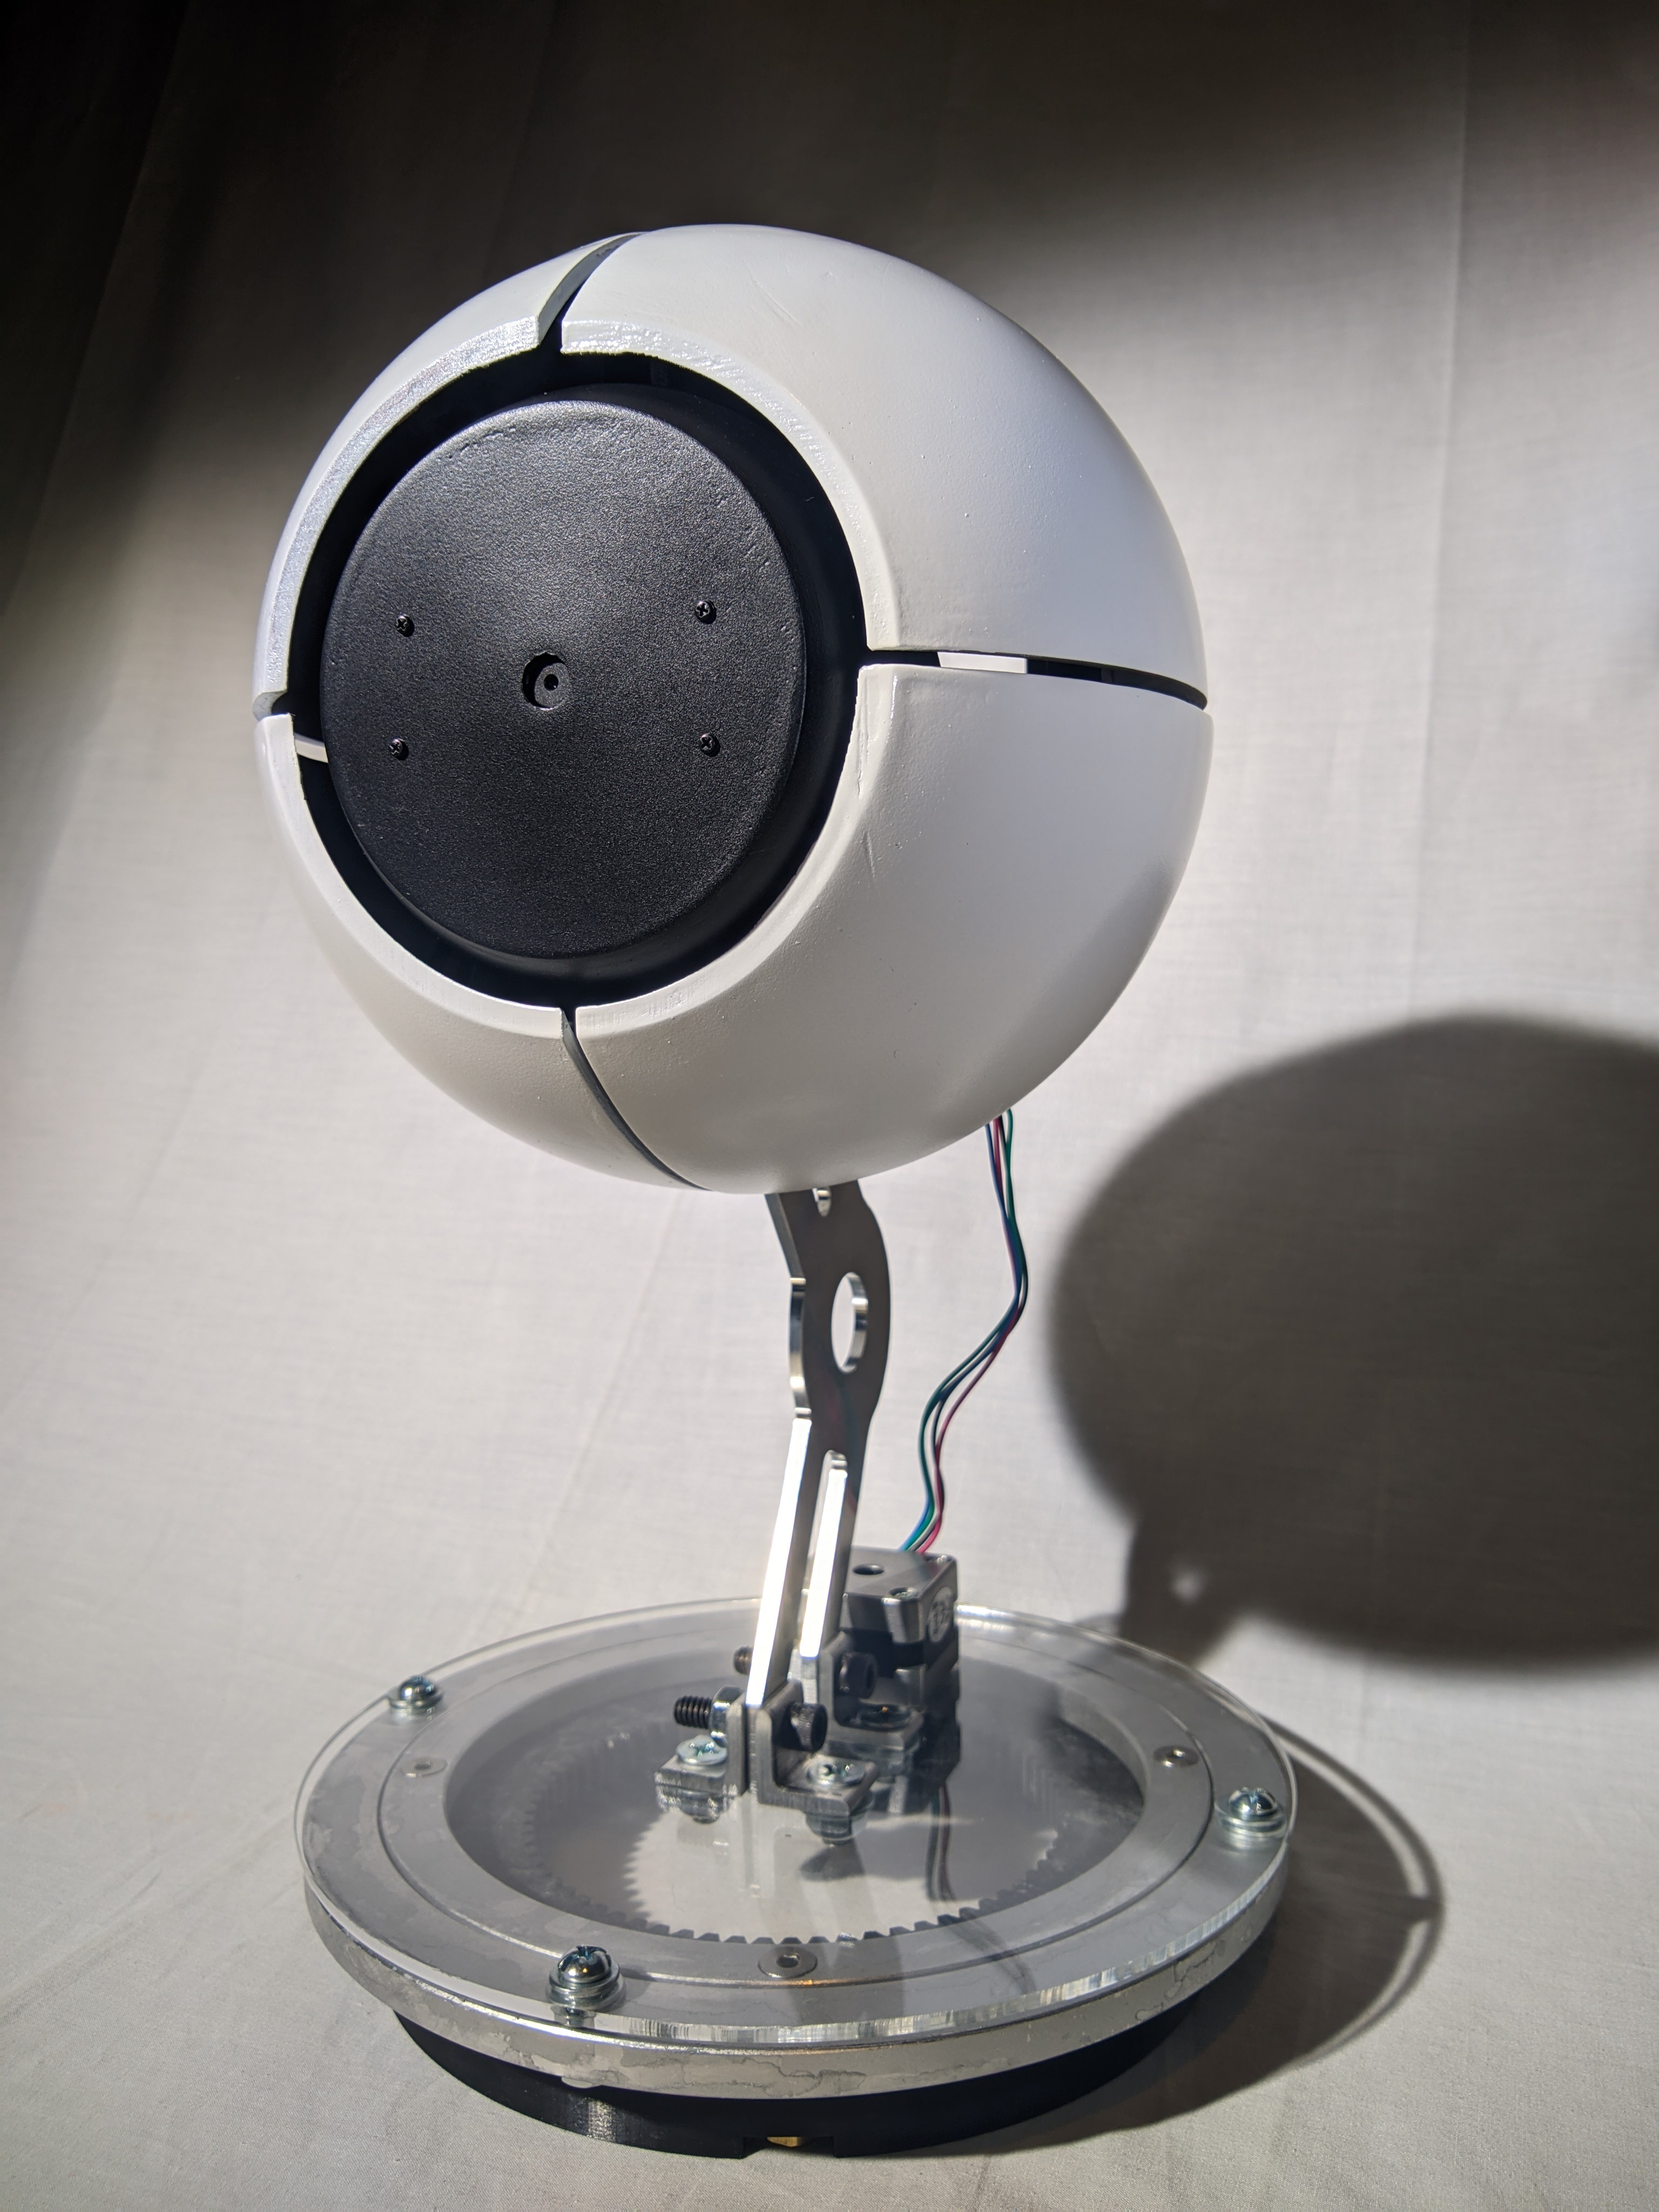
\includegraphics[width=0.6\linewidth]{Thesis/best-view.jpg}
    \caption{Photo of the final model.}
    \label{fig:final_model}
\end{figure}